\documentclass[conference]{IEEEtran}
\IEEEoverridecommandlockouts
% The preceding line is only needed to identify funding in the first footnote. If that is unneeded, please comment it out.
%Template version as of 6/27/2024

\usepackage{cite}
\usepackage{amsmath,amssymb,amsfonts}
\usepackage{algorithmic}
\usepackage{graphicx}
\usepackage{textcomp}
\usepackage{xcolor}
\usepackage[table]{xcolor}
\usepackage{enumitem}
\usepackage{booktabs}
\usepackage{url}
% hyperref intentionally NOT loaded: EDAS rejects PDFs containing hyperlinks/bookmarks.
% \url{} is provided by the url package above and renders as plain (non-clickable) text.
\usepackage{tabularx}
\usepackage{float}
% Sub-figures per the IEEEtran HOWTO (Sec. X-A-1). caption=false is required so
% that caption.sty does not take main-caption formatting away from IEEEtran.
\usepackage[caption=false,font=footnotesize]{subfig}
\def\BibTeX{{\rm B\kern-.05em{\sc i\kern-.025em b}\kern-.08em
    T\kern-.1667em\lower.7ex\hbox{E}\kern-.125emX}}

% --- Compact spacing (font sizes intentionally left unchanged) ---
% Reduces whitespace around floats, captions and equations only.
\setlength{\textfloatsep}{6pt plus 2pt minus 2pt}
\setlength{\floatsep}{6pt plus 2pt minus 2pt}
\setlength{\intextsep}{6pt plus 2pt minus 2pt}
\setlength{\abovecaptionskip}{4pt}
\setlength{\belowcaptionskip}{0pt}
\setlength{\abovedisplayskip}{4pt plus 2pt minus 2pt}
\setlength{\belowdisplayskip}{4pt plus 2pt minus 2pt}
\setlength{\abovedisplayshortskip}{2pt plus 1pt}
\setlength{\belowdisplayshortskip}{2pt plus 1pt}

\begin{document}

\title{Automated Component Recovery and Custom Kit Assembly System for Educational Circuit Kits}

\author{\IEEEauthorblockN{1\textsuperscript{st} Aman Mishra}
\IEEEauthorblockA{\textit{Computer Eng. and Informatics} \\
\textit{Middlesex University Dubai}\\
Dubai, UAE \\
a.mishra@mdx.ac.ae}
\and
\IEEEauthorblockN{2\textsuperscript{nd} Faseeh Mohammed}
\IEEEauthorblockA{\textit{Computer Eng. and Informatics} \\
\textit{Middlesex University Dubai}\\
Dubai, UAE \\
ff416@live.mdx.ac.uk}
\and
\IEEEauthorblockN{3\textsuperscript{rd} Judhi Prasetyo}
\IEEEauthorblockA{\textit{Computer Eng. and Informatics} \\
\textit{Middlesex University Dubai}\\
Dubai, UAE \\
j.prasetyo@mdx.ac.ae}
}

\maketitle

\begin{abstract}
Educational institutions issue circuit development kits, such as Arduino modules, for practical coursework, but returned kits often lack critical components and cannot be redistributed as complete sets. This paper proposes an automated robotic solution to this logistical and environmental inefficiency. Unlike traditional assembly systems that build standard products from uniform supply lines, the proposed system recovers components from existing, incomplete kits. A Python machine-vision system identifies available modules and communicates via TCP/IP with an EPSON RC8.0 simulator controlling a VT6-A901S 6-axis robot, enabling dynamic assembly of new kits from custom Bills of Quantities (BOQs) submitted for specific projects. The result is a flexible, waste-reducing system that gives students exactly the components their modules require.
\end{abstract}

\begin{IEEEkeywords}
Robotic Assembly, Machine Vision, Component Recovery, EPSON RC8.0, Automation, E-waste.
\end{IEEEkeywords}

\section{Introduction}
Practical electronics and robotics education relies heavily on development kits, typically built around microcontrollers such as the Arduino alongside sensors, actuators, and passive components. Although students are encouraged to keep these kits, many return them at the end of term, often with modules missing, damaged, or misplaced. Because the returned kits are incomplete, they cannot be re-issued to incoming students who need standard, comprehensive sets, so institutions accumulate partial kits, incurring unnecessary procurement costs and electronic waste.

Vision-guided robotic sorting is mature, but deployed systems assume an engineered supply: uniform workpieces singulated on a conveyor, lighting designed so that segmentation is trivial, and identity read from an applied barcode rather than from appearance \cite{luo2024}. Recovery is a different regime. The closest work to this problem classifies discarded educational project parts from an overhead camera with high accuracy, but stops at the image: its regions are axis-aligned and carry no orientation, and the manipulator remains future work \cite{chand2022}. Two capabilities therefore remain open---the resting angle a gripper needs to align to a rectangular module, and a demand specification, since sorting is driven by destination or by class rather than by what a consumer actually requires.

This project develops a robotic system that sorts returned components and dynamically rebuilds kits. By targeting project-specific requirements rather than rigid standard kit definitions, the system reallocates whatever components a returned kit contains to the students whose projects actually need them, even when generic parts are absent.

\section{Methodology}
\subsection{Evaluation of Existing Solutions}
Automated kitting and assembly are well established but almost exclusively designed for factory-stage production, typically using Delta and SCARA (Selective Compliance Assembly Robot Arm) robots to pick uniform components from controlled feeder lines. A representative installation sorts metal workpieces by size on a conveyor using an industrial 6-axis arm and a vision system whose reliability is explicitly conditioned on purpose-built backlighting, and resolves part identity through barcode recognition and a database lookup rather than from the component's own appearance \cite{luo2024}. Unfortunately, this option remains unavailable for returned components, which carry no such tag. Automated sortation is also used in large-scale waste management: facility-scale smart sortation systems combine real-time machine vision with air jets and Delta arms to recover valuable commodities, including e-waste, from mixed municipal solid waste \cite{amp}. These systems prove the efficacy of AI-guided robotic sorting for high-volume recovery, but operate at facility scale for gross sorting rather than the precise, project-specific kitting of delicate microelectronic modules needed in education.

These methodologies share one assumption: a continuous, uniform supply of new components. No widely adopted solution recovers loose, mixed components from partially depleted kits to build newly configured ones. Recent work on e-waste recovery stresses that salvaging used electronics differs fundamentally from original production: recovery is characterized by high uncertainty, as components may be damaged, randomly oriented, or missing \cite{saenz}. Deterministic factory automation is therefore insufficient for these Re-X (Recycling, Re-use, Remanufacturing) activities, motivating the flexible, data-driven approach proposed here.

The closest published work shares this premise, recovering electronic parts left over from student project work on circular-economy grounds \cite{chand2022}. It extracts regions with a deterministic pipeline---Canny, dilation, flood-filling and region measurement---then compares shallow, support-vector and convolutional classifiers on the resulting crops. Its regions are axis-aligned, so no resting angle is recovered; its pixel-to-world step is an axis-wise scale factor from four corner markers, applying no perspective correction; and the robotic pick-and-place is future work rather than demonstrated.

\subsection{Proposed Unique Approach}
The solution's differentiating factor is intelligent recovery and flexible kitting. Rather than having staff manually audit and sort thousands of components to rebuild standard kits, the system operates on a custom Bill of Quantities (BOQ) model: staff or students submit a project BOQ, and the system identifies the required parts from the pool of returned components and assembles a kit tailored to that project. This shifts the institution from a ``push'' model (a standard kit for everyone regardless of need) to a ``pull'' model (kits assembled strictly from project requirements), maximizing the utility of returned inventory.

\section{Implementation}
To realize this automated recovery and assembly system, a digital twin of the robotic workcell has been developed, integrating high-level software control with industrial robotic simulation containing accurate real world measurements and sensor readings.

\subsection{Machine Vision System}
\begin{figure}[!b]
  \centering
  \subfloat[]{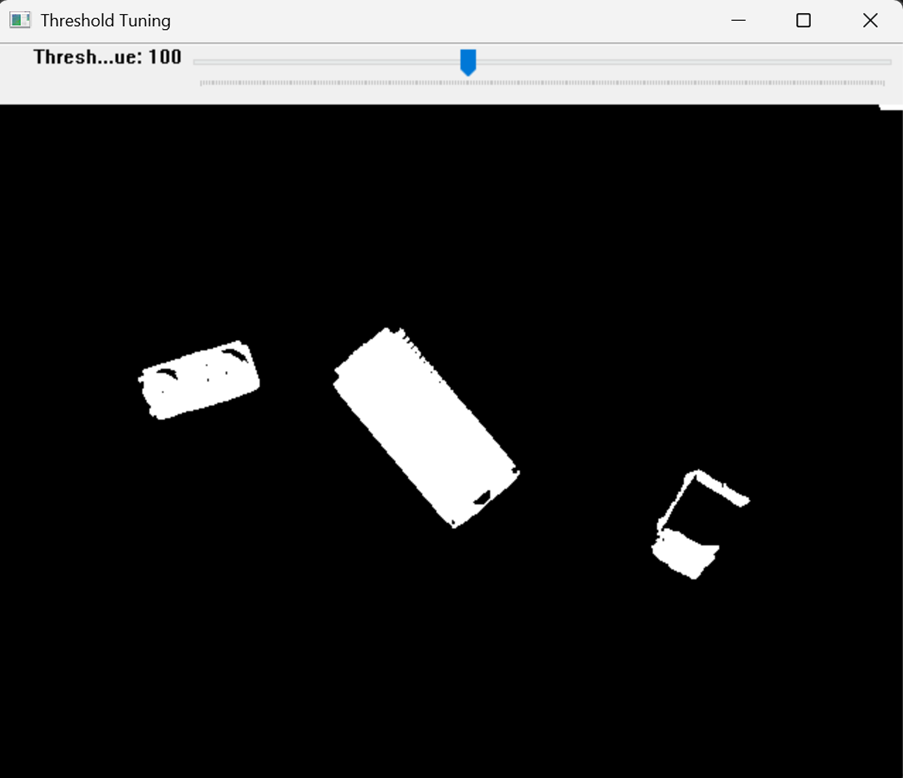
\includegraphics[height=0.45\columnwidth]{imgs/threshold_pickerbot.png}%
    \label{fig:thresholding}}
  \hfil
  \subfloat[]{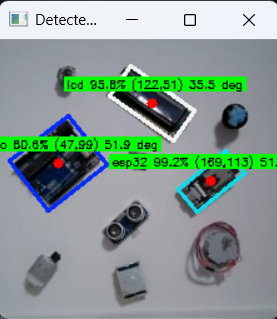
\includegraphics[height=0.45\columnwidth]{imgs/yolo_detect_v2.png}%
    \label{fig:yolo-detect}}
  \caption{Evolution of the perception stage, shown on comparable workbench
    scenes. (a) Prototype: global binary thresholding in OpenCV, tuned live by
    an operator slider. The mask isolates the three target modules but
    fragments them where glare erases surface texture, and carries no class or
    orientation information. (b) Deployed detector: YOLOv8-OBB inference on the
    raw frame, recovering class, confidence, centroid and resting angle for
    each module in a single forward pass while ignoring the surrounding
    clutter.}
  \label{fig:vision}
\end{figure}
The machine-vision architecture is the core of the pick-and-place operation: it scans the unstructured workbench, identifies components, decodes their orientation, and translates pixel data into Cartesian world coordinates for the manipulator. Many industrial bin-picking solutions rely on line-of-sight 3D cameras, but these generate point clouds prone to spurious outliers on cluttered, overlapping parts, degrading segmentation and obstacle-avoidance planning and requiring costly filtering \cite{Franaszek}. This project instead uses a 2D planar overhead approach, developed through two phases.

\subsubsection{Prototype Phase: Deterministic Computer Vision}
The initial architecture relied on deterministic OpenCV processing. Frames from an overhead 720p webcam were Gaussian-blurred, then global binary thresholding (Fig.~\ref{fig:thresholding}) isolated geometric footprints. Contour analysis (\texttt{cv2.findContours}) found each boundary, and a scale-preserving script padded the crops into uniform 224$\times$224 tensors for a Google Teachable Machine classifier. The prototype proved fragile despite being functional in controlled conditions. Metallic glare erased surface texture, while clutter and cast shadows produced spurious contours. A rotated rectangle fitted to each contour did recover a resting angle, but only ever as reliably as the mask beneath it. The pipeline also needed a separate five-class classifier per crop, and was superseded before the contour-to-classifier link was completed. Section~\ref{sec:baseline} quantifies these limits.

\subsubsection{Final Architecture: YOLOv8-OBB (Oriented Bounding Box)}
The system was therefore re-architected around a YOLOv8-OBB network ingesting the full-resolution, uncropped frame, eliminating manual thresholding and cropping. Trained on a purpose-built dataset annotated in the Computer Vision Annotation Tool (CVAT) under photometric and geometric augmentation (Section~\ref{sec:dataset}), the model bypasses glare and localized clutter (Fig.~\ref{fig:yolo-detect}). The manual annotation this supervised approach requires is a necessary trade-off for the recognition quality and spatial accuracy bin-picking demands \cite{Fager}. In one forward pass it outputs a 5-D oriented tensor \texttt{(cx, cy, width, height, theta)} with class probabilities. This is far simpler than hybrid pipelines using, for example, YOLOv5 top-view detection followed by an eye-in-hand FAST/BRISK step for pose estimation \cite{Taweesoontorn}; deriving theta from a single overhead frame removes any dependence on perfect lighting or multi-step capture.
\subsubsection{Dataset and Training Configuration}
\label{sec:dataset}
\begin{table}[b]
  \caption{Dataset and Training Configuration}
  \label{tab:training}
  \centering
  \footnotesize
  \begin{tabular}{@{}ll@{}}
    \toprule
    \textbf{Parameter} & \textbf{Value} \\
    \midrule
    \multicolumn{2}{@{}l}{\textit{Dataset}} \\
    Images (train / validation)      & 50 / 6 \\
    Instances (train)                & 132 (44 per class) \\
    Classes                          & Arduino, ESP32, LCD \\
    Annotation                       & CVAT, oriented bounding box \\
    Capture                          & Overhead 720p webcam, deployment cell \\
    \midrule
    \multicolumn{2}{@{}l}{\textit{Model and optimisation}} \\
    Network                          & YOLOv8n-OBB, COCO-pretrained \\
    Input resolution                 & $640 \times 640$ \\
    Epochs / batch size              & 100 / 16 \\
    Optimiser                        & AdamW (auto-selected) \\
    Learning rate (initial / final)  & $1.43{\times}10^{-3}$ / $1.43{\times}10^{-5}$ \\
    Schedule                         & Linear decay, 3 warm-up epochs \\
    Momentum / weight decay          & 0.9 / $5{\times}10^{-4}$ \\
    Loss weights (box/cls/dfl/angle) & 7.5 / 0.5 / 1.5 / 1.0 \\
    Training time                    & 151~s (Colab T4 GPU) \\
    \midrule
    \multicolumn{2}{@{}l}{\textit{Train-time augmentation}} \\
    HSV hue / saturation / value     & 0.015 / 0.7 / 0.4 \\
    Translation / scale              & 0.1 / 0.5 \\
    Horizontal flip / mosaic         & 0.5 / 1.0 (off for last 10) \\
    Random erasing                   & 0.4 \\
    Rotation / shear / perspective   & disabled \\
    \bottomrule
  \end{tabular}
\end{table}

Table~\ref{tab:training} lists the full configuration. The detector was trained on 56 overhead images captured with the deployment camera on the workcell itself, so training and operating distributions coincide by construction. Components were placed at varied positions and resting yaw angles, and oriented boxes for the three classes annotated in CVAT. The 50/6 train/validation split yields 132 training instances, balanced at 44 per class.

Training began from COCO-pretrained \texttt{yolov8n-obb} weights and ran 100 epochs at 640~px. Automatic optimiser selection resolved to AdamW at an initial learning rate of $1.43{\times}10^{-3}$, decayed linearly to one percent of that value over three warm-up and 97 training epochs. The default augmentation pipeline was applied---HSV jitter, mosaic (disabled for the final ten epochs), translation, scaling, horizontal flipping and random erasing. Rotational augmentation was deliberately disabled: orientation diversity comes from the physical placement of components during capture, which samples the true distribution of resting angles more faithfully than synthetic rotation of a fixed overhead view. The run completed in 151~s on a single Colab GPU.

\subsubsection{Logistics Filtering and BOQ Engine}
Once the vision system extracts each component's pixel centroid and class label, a logistics filter operates above the frame buffer. Rather than forwarding every detection to the coordinate-mapping pipeline, the orchestrator matches detected inventory against a Bill of Quantities (BOQ), ignoring surplus components even when validly detected, so only the required items reach the spatial calibration engine.


\subsection{Spatial Calibration and Coordinate Mapping}

\begin{figure}[b]
  \centering
  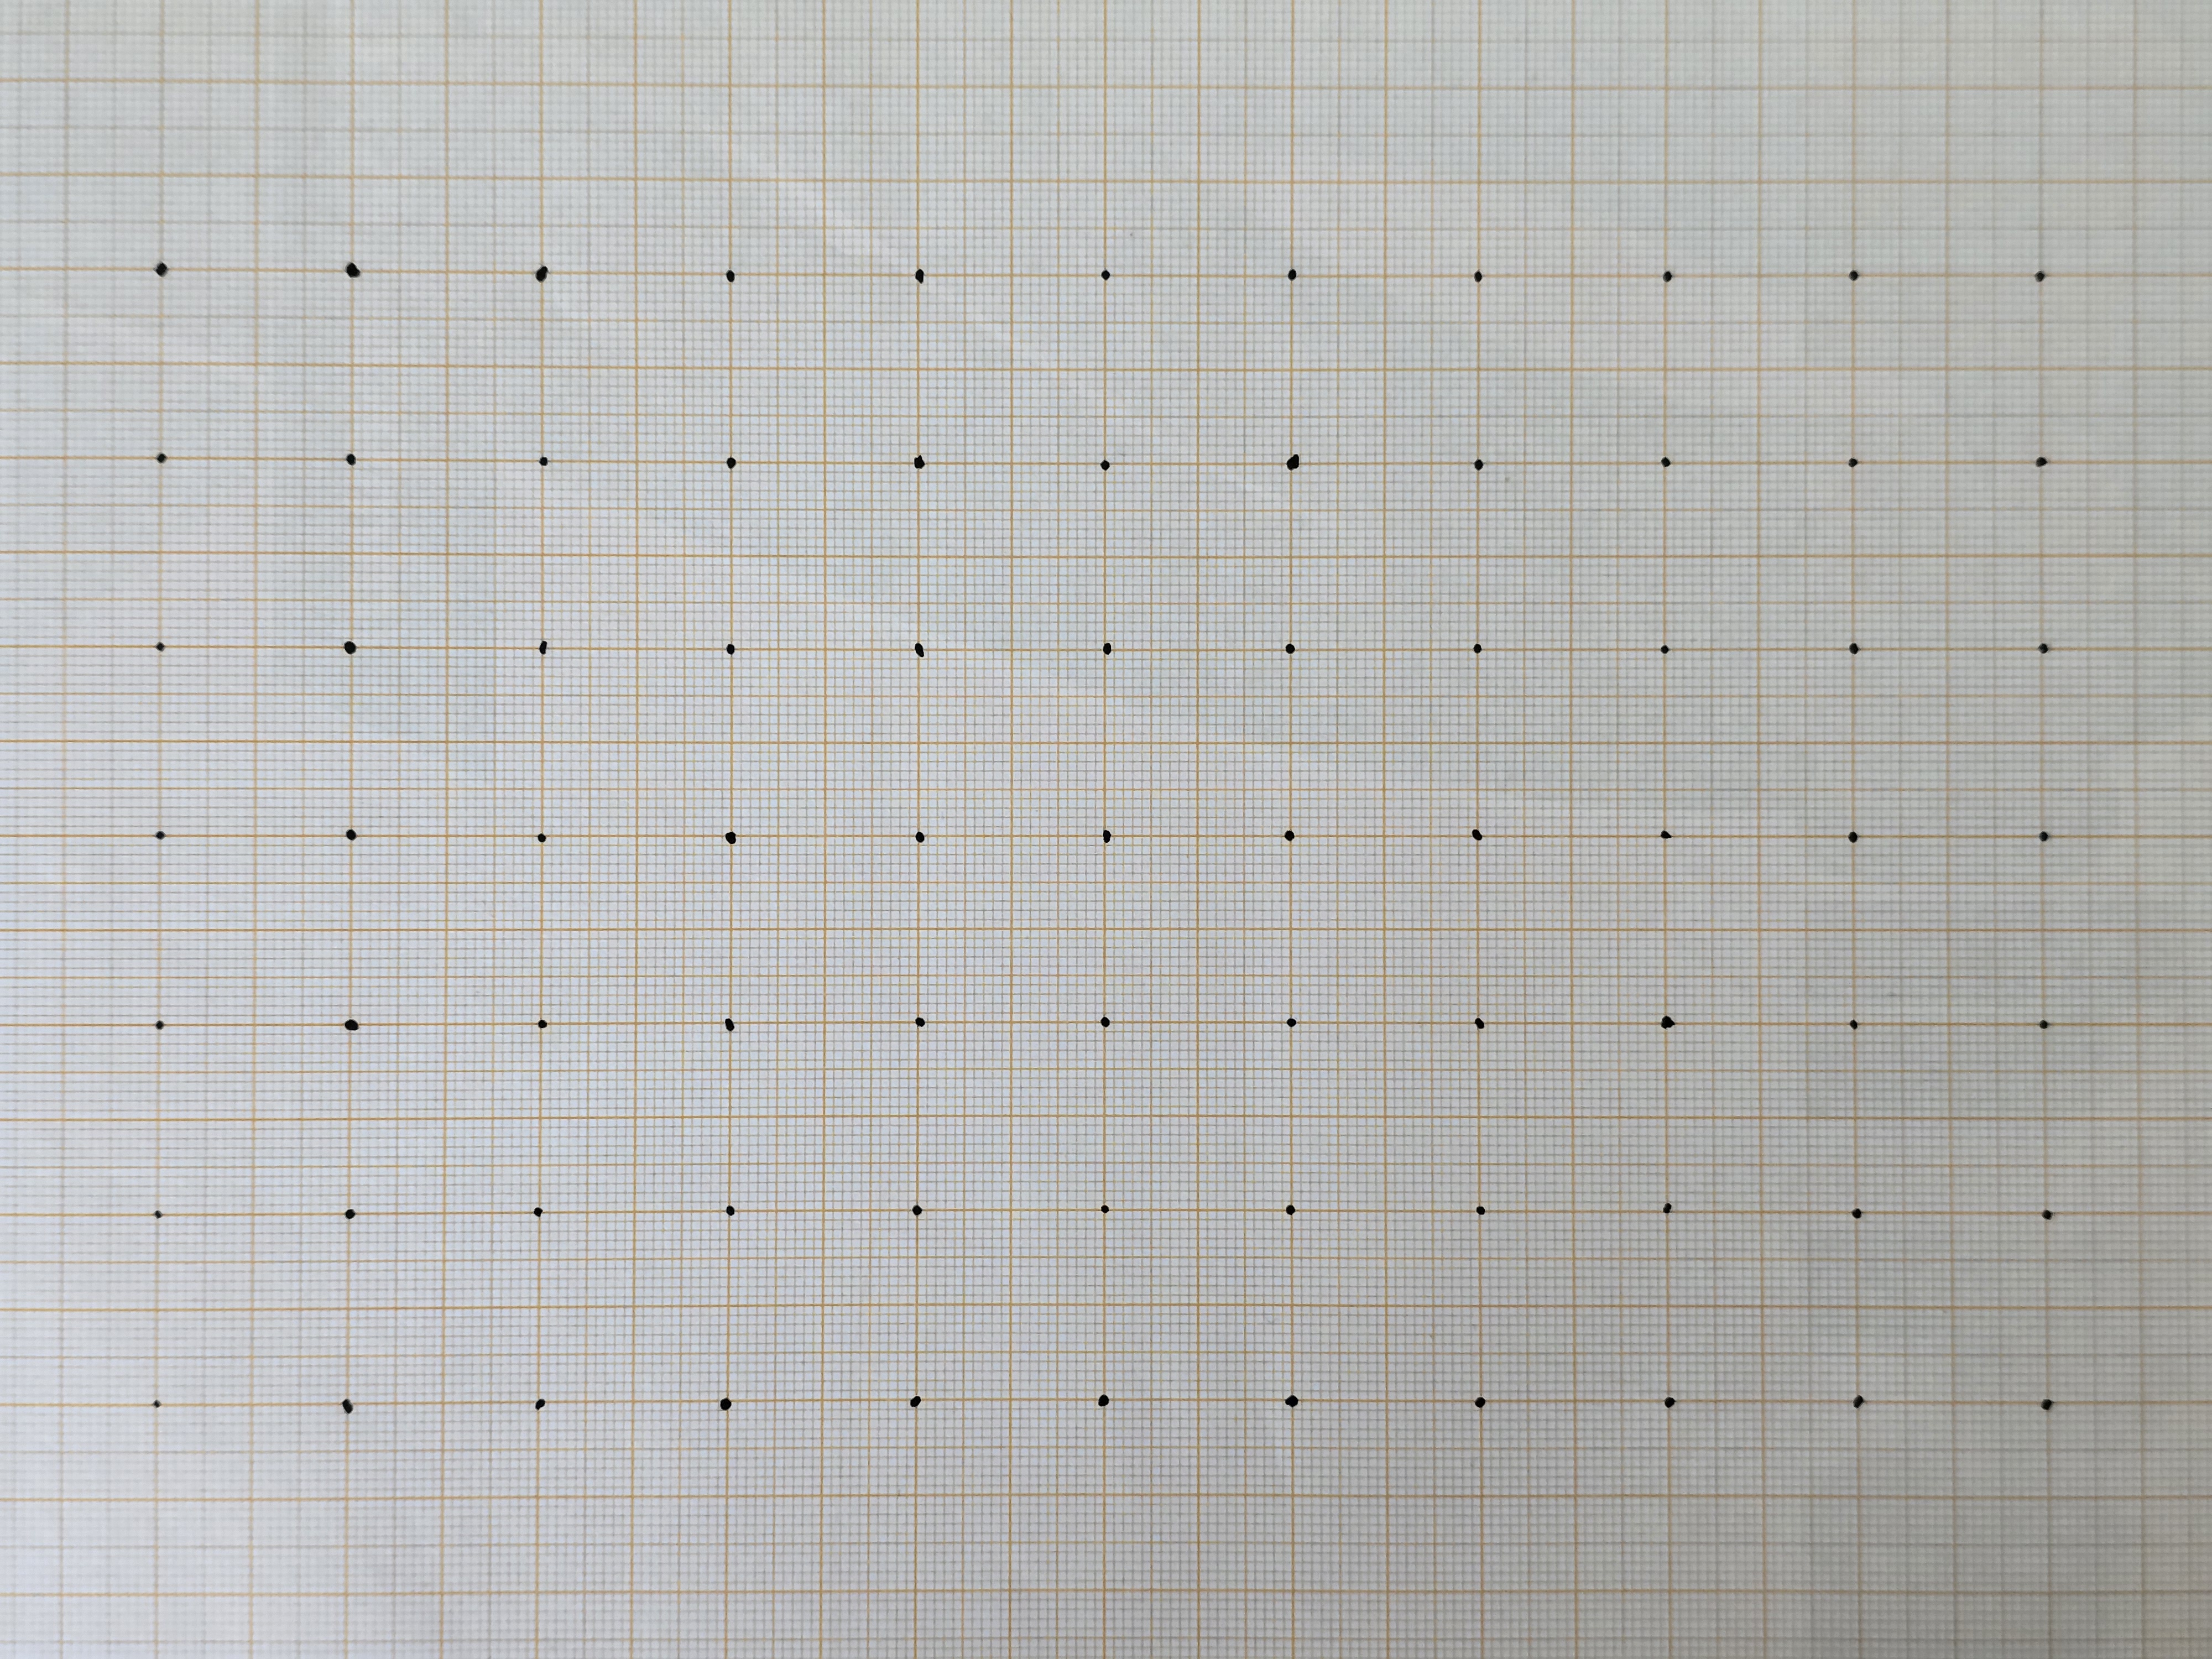
\includegraphics[width=0.66\columnwidth]{imgs/graph_paper.jpg}
  \caption{77-point homography calibration grid showing pixel click positions overlaid on the workspace reference image.}
  \label{fig:calibration_grid}
\end{figure}

Translating pixel positions into millimetre coordinates in the robot's world frame is achieved through a planar homography, a projective mapping between the two coordinate spaces.

The mapping uses a 77-point grid of 11 columns by 7 rows at 20~mm spacing (Fig.~\ref{fig:calibration_grid}). World X decreases from $+$100~mm to $-$100~mm left to right and world Y increases from 410~mm to 530~mm top to bottom, giving a calibrated area of 200~mm $\times$ 120~mm. A reference image is captured with the camera normal to the workspace; \texttt{calibration\_clicker.py} records the intersections and \texttt{sort\_and\_tag\_pixels.py} sorts them column by column, appending world coordinates to produce a pixel-to-world CSV.

The homography $\mathbf{H}$ is computed with OpenCV's \texttt{findHomography} using standard least squares (SLS), not RANSAC. This is deliberate: the corner points define the workspace extremes and are valid constraints, so rejecting them as outliers would introduce systematic error near the boundaries. With 77 evenly distributed points, SLS is robust without outlier rejection. At runtime each detected centroid is mapped via \texttt{cv2.perspectiveTransform}. $\mathbf{H}$ is a mapping of the bench plane alone, so every detected centroid is treated as coplanar with the calibration grid; no per-class height offset is applied, and modules of appreciable thickness therefore retain a residual lateral error addressed in Section~\ref{sec:limits}.

Repositioning the camera vertically rescales the image and invalidates the mapping. Rather than re-clicking all 77 intersections, a recalibration routine has the user mark two points a known 20~mm apart, from which
\begin{equation}
  s = \frac{d_{\mathrm{measured}}}{d_{\mathrm{expected}}},
  \qquad
  d_{\mathrm{expected}} = \sqrt{(r_h\cos\theta)^2 + (r_v\sin\theta)^2}
\end{equation}
is derived, with $r_h$ and $r_v$ the separate horizontal and vertical pixel pitches. This anisotropic form accommodates lens geometry and non-square sampling. All 77 coordinates are then scaled about the grid centre and cached.

\begin{figure}[b]
  \centering
  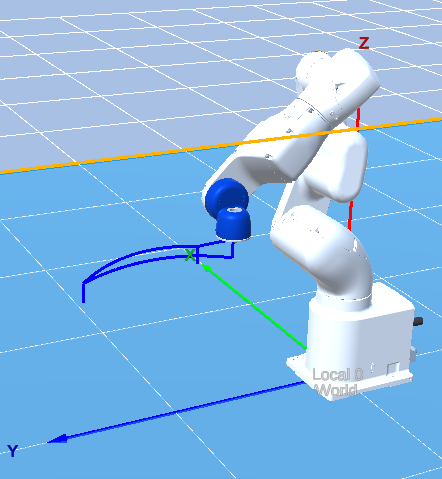
\includegraphics[width=0.68\columnwidth]{imgs/pick_trajectory.png}
  \caption{Trajectory of the \texttt{PICK} command: three-phase Jump3 approach to the component, gripper activation, transport to \texttt{PlacePoint}, and release.}
  \label{fig:pick_trajectory}
\end{figure}

\subsection{TCP/IP Communication Protocol}

Fig.~\ref{fig:pick_trajectory} shows a sample pick-and-place for one item: from standby, the arm approaches the object in the correct orientation, picks it, jumps to the place point, fixes orientation, places, and retracts to standby for the next operation.

The Python control system communicates with the EPSON RC8 controller over a local TCP socket (\texttt{127.0.0.1}:2001 in simulation, a LAN address for the physical robot). Commands are plain ASCII strings of the form \texttt{COMMAND~X~Y~Z~U\textbackslash r\textbackslash n}, where $X,Y,Z$ are world coordinates in millimetres and $U$ is the tool rotation in degrees. The supported set is \texttt{JUMP}, \texttt{GO}, \texttt{MOVE}, \texttt{PICK} and \texttt{STANDBY}; the controller replies \texttt{"OK"} after each, and a small inter-command delay allows mechanical completion before the next is sent.

For multi-component picks, \texttt{epsonPickAll} iterates over a list of world-coordinate strings and issues a \texttt{PICK} for each, checking the reply against \texttt{"OK"}. Any non-OK response aborts the batch immediately and returns the robot to standby, so a partial failure such as a grip error or controller fault cannot leave the robot operating in an undefined state.

\subsection{EPSON RC8 Robot Program}
\label{sec:epson}

\texttt{Epson/Pickerbot\_Receiver/Main.prg}, the robot-side program is written in Epson SPEL+, the RC8 controller's scripting language, building on a template script \cite{prasetyo2024} with predefined motion-initialization parameters. After initialization it opens a TCP server on channel \#201 at port 2001 and waits for a client before entering its command loop.

Each string is split on spaces into a command token and floating-point arguments. \texttt{PICK} is the most complex: a three-phase Jump3 trajectory lifts the arm vertically, translates to an elevated waypoint above $(x, y)$ with the tool at orientation $u$, and descends to the pick position, where a digital output closes the gripper and a dwell ensures a reliable grip. A second Jump3 lifts clear and transports the component to a predefined \texttt{PlacePoint}, where the output is deactivated to release it before the arm returns to standby. A network error handler reopens the socket and resumes listening rather than halting, letting the system recover from transient interruptions without operator intervention.

\begin{figure}[b]
  \centering
  \includegraphics[width=0.89\columnwidth]{imgs/software_architecture_v2.png}
  \caption{Software architecture of the Picker-Bot system, illustrating the three entry-point scripts and their shared dependency on the \texttt{pickerbot\_lib} package.}
  \label{fig:architecture}
\end{figure}

\subsection{Software Architecture and Entry Points}

The codebase (Fig.~\ref{fig:architecture}) is built around a shared package, \texttt{pickerbot\_lib}, consolidating detection, calibration, and TCP communication into three submodules: \texttt{detection}, \texttt{calibration}, and \texttt{sender}. Three entry-point scripts at the project root each import this package to serve a distinct mode.

The primary entry point, \texttt{pickerbot.py}, orchestrates an end-to-end pick session: \texttt{{-}{-}src} selects the detection source (live camera or static image) and \texttt{{-}{-}calibrate} launches the height-recalibration GUI. In a normal run it loads the homography CSV named in \texttt{config.json}, runs detection, maps each centroid to world coordinates and dispatches the list to \texttt{epsonPickAll}. The second, \texttt{detect\_and\_classify.py}, isolates the vision layer for testing without a robot: given a file path it processes a static image, and without arguments opens the live feed with a confidence-threshold slider. The third, \texttt{teleop\_mouse.py}, provides interactive positioning, displaying the reference image with all 77 points annotated and sending each click through $\mathbf{H}$ as a \texttt{MOVE} command---useful for verifying calibration accuracy before an automated session.

\subsection{Robotic Control and Simulation}
Manipulation is done in a simulated digital twin in the EPSON RC8.0 environment. While the system can cover any workspace size, the initial setup mapped a 200~mm $\times$ 120~mm evaluation space with a deposit point 280~mm above its centre. The platform is the EPSON VT6-A901S~\cite{b2}, a 6-axis arm with 980~mm reach suited to pick-and-place requiring varied approach angles and high repeatability; full installation, safety, and operational specifications appear in the Epson VT6 documentation \cite{epsonvt6}. The arm is existing teaching-laboratory equipment, and the system was built around the hardware already available rather than around a purpose-selected platform. Additionally, since the control interface assumes that the controller accepts Cartesian targets over a socket, the pipeline transfers unchanged to manipulators of different reach and cost, provided the target controller exposes a Cartesian interface or an inverse-kinematics solver to resolve the joint angles; verifying this on other platforms is beyond the scope of this paper. The end effector is modelled only as the binary digital output and fixed dwell described in Section~\ref{sec:epson}: no jaw or suction geometry is configured, so the Jump3 clearances and dwell are trajectory-level parameters rather than values validated against a physical tool. Selecting that tool, and with it the payload and approach constraints it imposes, belongs to physical deployment.

\section{Results}
The following subsections report observed behaviour across three layers: perception, spatial reasoning, and supervised manipulation.

\subsection{Detection Performance}

\begin{table}[b]
  \caption{Quantitative Evaluation}
  \label{tab:eval}
  \centering
  \footnotesize
  \begin{tabular}{@{}lccccc@{}}
    \toprule
    \multicolumn{6}{@{}l}{\textit{(a) Detection --- validation split, 6 images / 18 instances}} \\
    Class & Inst. & P & R & $mAP_{50}$ & $mAP_{50\text{--}95}$ \\
    \midrule
    Arduino & 6 & 0.977 & 1.000 & 0.995 & 0.995 \\
    ESP32   & 6 & 1.000 & 1.000 & 0.995 & 0.955 \\
    LCD     & 6 & 0.975 & 1.000 & 0.995 & 0.971 \\
    \textbf{All} & \textbf{18} & \textbf{0.984} & \textbf{1.000} & \textbf{0.995} & \textbf{0.974} \\
    \midrule
    \multicolumn{6}{@{}l}{\textit{(b) Vision throughput --- per frame}} \\
    \multicolumn{4}{@{}l}{Pre-process / inference / post-process} & \multicolumn{2}{r@{}}{0.3 / 13.9 / 2.7~ms} \\
    \multicolumn{4}{@{}l}{Total}                                  & \multicolumn{2}{r@{}}{16.9~ms (59~fps)} \\
    \bottomrule
  \end{tabular}
\end{table}

The migration to YOLOv8-OBB substantially improved detection reliability. The final model classified Arduino, ESP32 and LCD modules and recovered the resting angle $\theta$ with the centroid $(cx, cy)$ in a single forward pass without geometric post-processing, absorbing the glare, clutter and background texture that had destabilised the prototype. The explicit reject class the prototype classifier required became unnecessary: the detector trains on the three component classes alone and treats everything else as background, so spurious regions are rejected by the confidence threshold rather than a dedicated reject class.

Table~\ref{tab:eval}(a) reports per-class validation metrics. The model reached an $mAP_{50}$ of 0.995 at 1.000 recall and 0.984 precision, with a fully diagonal normalised confusion matrix: no inter-class confusion and no component predicted as background. The $mAP_{50\text{--}95}$ of 0.974 matters more because OBB matching uses \emph{rotated} intersection over union (IoU)---a detection whose yaw is substantially wrong fails to match at the higher IoU thresholds---so a high value certifies that the recovered angle $\theta$, not merely the class label, is accurate. Convergence was rapid: $mAP_{50}$ exceeded 0.99 by epoch~7 and $mAP_{50\text{--}95}$ passed 0.90 by epoch~17, the remainder refining localisation. A fixed confidence threshold of 0.65 eliminated the few glare-induced false positives, with no additional non-maximum suppression.

Perception is not the throughput bottleneck. End-to-end vision cost is 16.9~ms per frame (Table~\ref{tab:eval}(b)), around 59~fps; cycle time is dominated by the Jump3 trajectory and the fixed inter-command delay discussed in Section~\ref{sec:limits}.

\subsubsection*{Scope of this evaluation}
The validation split contains 6 images and 18 instances. No separate test partition was withheld, so the images measuring performance also informed checkpoint selection. These figures are therefore an in-distribution characterisation of the deployment cell, not an estimate of generalisation. At this sample size a recall of 18/18 carries a 95\% Wilson interval of $[0.82, 1.00]$, and precision cannot resolve differences of a few percent; the interval, rather than the point estimate, is the honest summary. A single 50/6 split is also a poor estimator at this scale: $k$-fold cross-validation over the pooled 56 images would condition the estimate far better, and is planned for physical deployment alongside a capture session withheld in full.

\subsection{Spatial Calibration and Mapping Accuracy}
\label{sec:spatial}

The homography reliably bridged image and workspace, the 77-point grid defining a calibrated region of roughly $200~\text{mm} \times 120~\text{mm}$ covering the full overhead field of view. Using SLS rather than RANSAC kept the boundary corners from being discarded as outliers, which would have contracted that area. Height recalibration absorbed camera repositioning in seconds without re-clicking every intersection, and was verified through \texttt{teleop\_mouse.py}, where each click produced a \texttt{MOVE} command whose terminal position visually matched the clicked feature.

\subsection{Comparison with the Deterministic Baseline}
\label{sec:baseline}

\begin{table}[b]
  \caption{Deterministic Baseline vs.\ YOLOv8-OBB, Five Workbench Scenes}
  \label{tab:baseline}
  \centering
  \footnotesize
  \begin{tabular}{@{}lcc@{}}
    \toprule
                                        & Threshold\,+\,contour & YOLOv8-OBB \\
    \midrule
    Scenes correct, per-scene tuning    & 5 / 5                 & --- \\
    Scenes correct, one global setting  & 4 / 5                 & 5 / 5 \\
    Stable parameter window             & narrows with clutter  & conf.\ 0.20--0.44 \\
    Spurious regions at best setting    & 3                     & 0 \\
    Class label                         & separate classifier   & joint \\
    Orientation $\theta$                & fitted to mask        & regressed \\
    \bottomrule
  \end{tabular}
\end{table}

To quantify why the deterministic pipeline was abandoned, it was re-run alongside the deployed detector on five held-out workbench scenes containing 1--11 components each. The comparison is not merely historical: deterministic segmentation of this class, governed by a single global parameter, remains the detection stage of recent component-recovery work \cite{chand2022}. The contour stage's area bounds were scaled proportionally to image area from the values used at 720\,p, and the binary threshold was swept across its full range, so the baseline is credited with its best achievable result rather than one arbitrary setting.

Table~\ref{tab:baseline} summarises the outcome. Given per-scene tuning, the baseline recovers the correct region count in all five scenes, but no single threshold serves them all. The best global value succeeds on four and over-segments the fifth into 14 regions against 11 true components, the surplus being glare and shadow. The usable window also collapses with clutter---130 of 255 values for one component, 74 for four, and 15 and 8 for the two eleven-component scenes---requiring manual retuning between scenes.

The learned detector behaves in the opposite way. Any fixed confidence between 0.20 and 0.44 recovers all 13 target-class instances across all five scenes with no false positives; the deployed value of 0.65 recovers 12 of 13, the single miss being an ESP32 returned at 0.444 confidence rather than a localisation failure. The difference is parameter stability rather than peak accuracy: one confidence value transfers unchanged across every scene. The baseline is also class-agnostic, proposing unlabelled regions that would require a separate classifier, which was never implemented.

\subsection{Integrated Robot Control and Logistics}
The control pipeline executed the pull-based kitting end-to-end. Given a BOQ, the system satisfied its requirements in order of detection confidence and ignored correctly recognised but unneeded components, behaving as a logistics auditor rather than a greedy collector; without a BOQ it reverted to greedily picking every detection above threshold.

The TCP/IP interface dispatched the full command set (\texttt{JUMP}, \texttt{GO}, \texttt{MOVE}, \texttt{PICK}, \texttt{STANDBY}) reliably across extended runs, each validated by an \texttt{OK} reply before the next was sent. The \texttt{PICK} primitive executed its three-phase Jump3 trajectory in every trial, and synthetic failures exercised the abort path, returning the manipulator to standby rather than continuing through an undefined state. These are functional verifications of the control layer in simulation rather than a measured grasp-success rate, which requires the physical cell (Section~\ref{sec:limits}).
\section{Conclusion and Future Work}
The Picker-Bot system shifted component kitting from a ``push'' model to a project-specific ``pull'' model. Its cornerstone was the migration from deterministic OpenCV prototypes to YOLOv8-OBB: where the prototype was highly sensitive to environmental shifts, the final model reached an $mAP_{50}$ of 0.995 and an $mAP_{50\text{--}95}$ of 0.974 on an in-distribution validation split, while the 77-point homography mapped the full overhead field of view onto the workspace, showing that oriented bin-picking is viable in cluttered educational settings without 3D point-cloud hardware. Filtering detections through the BOQ engine lets the system both detect parts and manage inventory, addressing the goal of reducing procurement costs and e-waste. These are the two capabilities prior recovery work left open: the oriented detector supplies the resting angle axis-aligned classification cannot, and the BOQ engine supplies the demand specification destination-driven sorting does not model.
\subsection{Limitations}
\label{sec:limits}
Three limits bound what the reported numbers support. The detector was evaluated on a 6-image, 18-instance validation split drawn from the same capture session as the training data and not withheld from checkpoint selection, so it characterises in-distribution accuracy in the deployment cell rather than generalisation; a held-out session, and ideally a second lighting configuration, is the next measurement to take. Separately, the manipulation layer is verified functionally in simulation but its grasp-success rate is not quantified, since a meaningful figure requires the physical robot and real components. Finally, the detector covers three module classes, reflecting the dataset assembled rather than a ceiling of the architecture, since additional classes require only an extended annotation set and no change to the network or the downstream pipeline.

Three further constraints would affect any physical deployment. The fixed delay after each \texttt{OK} kept the simulated pipeline stable but should be tuned per component, since a heavier LCD settles differently from an ESP32 and one value trades throughput against reliability. The homography is a planar model of a three-dimensional problem: components of non-negligible height introduce a parallax offset appearing as systematic lateral error during the Jump3 descent, so a height-aware correction---per-class offsets or a depth sensor---would be needed. Finally, abort-on-failure, correct as an industrial default, is blunt at higher throughputs, where distinguishing transient communication faults from mechanical errors would be necessary to scale.
\subsection{Future Work}
Addressing these limits begins with deployment to physical hardware, which requires calibrating the camera under varying lighting, tuning gripper timing to real component dynamics, and likely an adaptive or compliant gripper for delicate modules. Further ahead, a web portal would let students submit BOQs and collect completed kits directly, while Internet of Things technologies and Autonomous Guided Vehicles, increasingly used to route materials in flexible manufacturing \cite{vlachos}, could fetch bins of returned kits to the workcell and deliver finished kits to collection points.

\subsection{Concluding Remarks}
The Picker-Bot system provides a technically sound, sustainable solution for managing returned educational circuit kits. By integrating Oriented Bounding Box detection, planar homography, and TCP/IP control, it shows that modern AI can turn ``loose waste'' into project-ready assets, setting a precedent for ``Re-X'' (Recovery and Re-use) activities in microelectronic environments and bridging waste management with logistical efficiency.
\section*{Acknowledgment}
The authors acknowledge the guidance and resources of the PDE4435 module, which encouraged a design-thinking approach to advanced robotics projects, Bilal Baslar for recommending the YOLOv8-OBB architecture adopted in Phase 2, and the use of Claude Code to set up the baseline masking filters for detection with sliders for human-operated tuning before transitioning to YOLOv8-OBB.

\begin{thebibliography}{00}
\bibitem{luo2024}
Y. Luo, ``Research on sorting system of industrial robot based on machine vision,'' in \textit{Proc. 2024 Int. Conf. Power, Electrical Engineering, Electronics and Control (PEEEC)}, 2024, pp. 270--274.
\bibitem{chand2022}
P. Chand and S. Lal, ``Vision-based detection and classification of used electronic parts,'' \textit{Sensors}, vol. 22, no. 23, p. 9079, Nov. 2022.
\bibitem{amp}
AMP, ``AMP ONE: Automated Waste Sorting Systems \& Facility,'' 2026. [Online]. Available: \url{https://ampsortation.com/products/amp-one}. [Accessed: Apr. 17, 2026].
\bibitem{saenz}
J. Saenz \textit{et al.}, ``Automated disassembly of e-waste---requirements on modeling of processes and product states,'' \textit{Frontiers in Robotics and AI}, vol. 11, p. 1303279, 2024.
\bibitem{Franaszek}
M. Franaszek, P. Rachakonda, and K. S. Saidi, ``Filtering organized 3D point clouds for bin picking applications,'' \textit{Applied Sciences}, vol. 14, no. 3, p. 961, Jan. 2024.
\bibitem{Fager}
P. Fager, R. Hanson, \text{\AA}. Fasth-Berglund, and S. Ekered, ``Supervised and unsupervised learning in vision-guided robotic bin picking applications for mixed-model assembly,'' \textit{Procedia CIRP}, vol. 104, pp. 1304--1309, 2021.
\bibitem{Taweesoontorn}
T. Taweesoontorn, S. Yanyong, and P. Konghuayrob, ``Hybrid deep learning and FAST--BRISK 3D object detection technique for bin-picking application,'' \textit{Sensors and Materials}, vol. 36, no. 4, pp. 1389--1404, 2024.
\bibitem{prasetyo2024}
J. Prasetyo, ``RC7\_Python,'' Jan. 03, 2024. Available: \url{https://github.com/judhi/RC7_Python}. [Accessed: Apr. 07, 2026].
\bibitem{b2} EPSON Robotics, ``RC8.0 reference manual,'' EPSON Factory Automation, 2023. [Online]. Available: \url{https://www.epson.com}. [Accessed: Apr. 07, 2026].
\bibitem{epsonvt6}
Epson America, Inc., ``Epson VT6L all-in-one 6-axis robots | support,'' Epson US, 2026. [Online]. Available: \url{https://epson.com/Support/Robots/6-Axis-Robots/VT-Series/Epson-VT6L-All-in-One-6-Axis-Robots/s/SPT_VT6L-A901SS}. [Accessed: Apr. 07, 2026].
\bibitem{vlachos}
I. Vlachos, R. M. Pascazzi, M. Ntotis, K. Spanaki, S. Despoudi, and P. Repoussis, ``Smart and flexible manufacturing systems using Autonomous Guided Vehicles (AGVs) and the internet of things (IoT),'' \textit{International Journal of Production Research}, pp. 1--22, 2022.
\end{thebibliography}

\end{document}